\section{Le LHC: \emph{Large Hadron Collider}}\label{chapter-LHC-section-LHC}
\begin{wrapfigure}{R}{8.5cm}
\centering
\begin{tikzpicture}
\node[anchor=south west,inner sep=0] at (0,0) {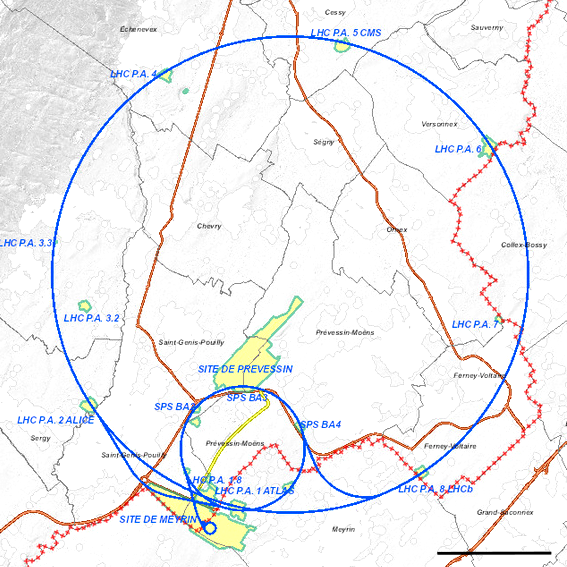
\includegraphics[scale=.35]{\PhDthesisdir/slides/LHC-CMS/LHC/CERN_LHC_map-scale_2km.png}};
\draw (6.125,.4) node {\SI{2}{\kilo\meter}};
\draw (2.95,.75) coordinate (LHCp1);
\draw (1.125,2) coordinate (LHCp2);
\draw (.65,4) coordinate (LHCp3);
\draw (1,3.2) coordinate (LHCp32);
\draw (2,6.1) coordinate (LHCp4);
\draw (4.25,6.45) coordinate (LHCp5);
\draw (6.05,5.15) coordinate (LHCp6);
\draw (6.15,3.125) coordinate (LHCp7);
\draw (5.15,1.15) coordinate (LHCp8);
\draw (LHCp1) coordinate (ATLAS);
\draw (LHCp2) coordinate (ALICE);
\draw (LHCp5) coordinate (CMS);
\draw (LHCp8) coordinate (LHCb);

%\foreach \coord in {1,2,3,4,5,6,7,8,32}{
%\fill[ltcolorred] (LHCp\coord) circle (3pt);
%}

%\draw [ultra thick, ltcolorred] (3.575,3.625) circle (2.95) ;
%\draw [ultra thick, ltcolorred] (3,1.475) circle (.75) ;
%\draw [ultra thick, ltcolorred] (2.6,.5) circle (.075) ;
%\fill [ltcolorred] (2.55,.55) circle (.05) ;
%\draw [ultra thick, ltcolorred] (2.5,.5) --+ (-60:.15) ;
\end{tikzpicture}
\caption[Tracés des \emph{booster}, PS, SPS et du LHC.]{Tracés des \emph{booster}, PS, SPS et du LHC~\cite{CERN_map}.}
\label{fig-CERN_map}
\end{wrapfigure}
Le Grand Collisionneur de Hadrons~\cite{LHC_paper1,LHC_paper2,LHC_paper3} (LHC, \emph{Large Hadron Collider}) est le plus grand et le plus puissant accélérateur de particules au monde.
Son tracé ainsi que ceux du PS, du SPS et du \emph{Booster} sont illustrés sur la figure~\ref{fig-CERN_map}.
Le LHC est installé dans le même tunnel que le LEP, il s'agit donc d'un accélérateur circulaire de \SI{27}{\kilo\meter} de circonférence, situé entre \num{50} et \SI{100}{\meter} sous la frontière franco-suisse.
\par Le LHC permet de réaliser des collisions proton-proton, proton-ion lourd et ion lourd-ion lourd.
Les collisions d'ions lourds permettent de reproduire les conditions des premiers instants de l'Univers après le \emph{Big Bang} et sont principalement étudiée par l'expérience ALICE, une des quatre expériences du LHC présentées dans la section~\ref{chapter-LHC-section-LHC-subsec-experiments}.
Dans tous les cas, deux faisceaux de particules sont accélérés en sens inverses.
Dans le cadre de cette thèse, seules les collisions de protons sont considérées.
\par \todo{Run I, II, III ...}
\subsection{Accélération de protons}\label{chapter-LHC-section-LHC-subsec-pp_acceleration}
Les protons sont obtenus par ionisation de dihydrogène, directement issu d'une bouteille.
Les protons sont alors progressivement accélérés à travers différentes installations du CERN, illustrées sur la figure~\ref{fig-chapter-LHC-section-CERN-CERN_Accelerator-Complex}, menant les protons à des niveaux d'énergie de plus en plus hauts avant de pouvoir être injectés dans le LHC~\cite{LHC_paper3}:
\begin{itemize}
\item l'accélérateur linéaire 2 (LINAC~2)\footnote{Le LINAC~2 est remplacé pour le Run~III du LHC par le LINAC~4.} permet d'accélérer les protons à une énergie de \SI{50}{\MeV};
\item le \emph{Booster}, premier élément circulaire, amène les protons à \SI{1.4}{\GeV};
\item le PS permet d'atteindre \SI{25}{\GeV};
\item le SPS, dernier élément avant le LHC, accélère les protons jusqu'à \SI{450}{\GeV}.
\end{itemize}
Le LHC accélère alors les protons jusqu'à \SI{6.5}{\TeV} lors du Run~II et ira jusqu'à \SI{7}{\TeV} lors du Run~III, permettant de réaliser des collisions avec des énergies dans le centre de masse de \num{13} et \SI{14}{\TeV}, respectivement.
\subsection{Collisions de protons}\label{chapter-LHC-section-LHC-subsec-pp_collisions}

\subsection{Luminosité et nombre d'événements}\label{chapter-LHC-section-LHC-subsec-lumi}

\subsection{L'empilement}\label{chapter-LHC-section-LHC-subsec-PU}

\subsection{Les expériences du LHC}\label{chapter-LHC-section-LHC-subsec-experiments}
Quatre grandes expériences sont présentes sur le LHC. Elles se situent chacune à un des points d'interaction de l'anneau afin d'étudier les collisions qui y sont produites.
\begin{description}
\item[ALICE]\cite{alice_paper}, \emph{A Large Ion Collider Experiment}, est une expérience conçue pour étudier le déconfinement des quarks et des gluons à l'aide de collisions d'ions lourds. Ces études permettent de mieux comprendre le fonctionnement de la chromodynamique quantique ou QCD. Elle est installée au point~2 et réutilise l'aimant de l'expérience L3 du LEP.
\item[ATLAS]\cite{atlas_paper}, \emph{A Toroidal LHC ApparatuS}, est une expérience généraliste avec un éventail d'études très large, allant des mesures de précision des paramètres du modèle standard à la recherche de nouvelle physique. Ce détecteur se trouve au point~1 du LHC.
\item[CMS]\cite{cms_paper}, \emph{Compact Muon Solenoid}, est également une expérience généraliste dont les objectifs sont similaires à ceux d'ATLAS. Les détecteurs d'ATLAS et de CMS étant conçus différemment, ces deux expériences peuvent valider leurs résultats de manière indépendante. Le détecteur CMS est installé au point~5 du LHC, à l'exact opposé d'ATLAS.
\item[LHCb]\cite{lhcb_paper}, \emph{Large Hadron Collider beauty}, se concentre sur l'étude de la violation de la symétrie CP avec le quark~\quarkb, qui lui donne son nom. Cette expérience réalise également des mesures de précision de certains paramètres du modèle standard. L'expérience LHCb se situe au point~8.
\end{description}
